\documentclass[floatsintext,man]{apa6}

\usepackage{amssymb,amsmath}
\usepackage{ifxetex,ifluatex}
\usepackage{fixltx2e} % provides \textsubscript
\ifnum 0\ifxetex 1\fi\ifluatex 1\fi=0 % if pdftex
  \usepackage[T1]{fontenc}
  \usepackage[utf8]{inputenc}
\else % if luatex or xelatex
  \ifxetex
    \usepackage{mathspec}
    \usepackage{xltxtra,xunicode}
  \else
    \usepackage{fontspec}
  \fi
  \defaultfontfeatures{Mapping=tex-text,Scale=MatchLowercase}
  \newcommand{\euro}{€}
\fi
% use upquote if available, for straight quotes in verbatim environments
\IfFileExists{upquote.sty}{\usepackage{upquote}}{}
% use microtype if available
\IfFileExists{microtype.sty}{\usepackage{microtype}}{}

% Table formatting
\usepackage{longtable, booktabs}
\usepackage{lscape}
% \usepackage[counterclockwise]{rotating}   % Landscape page setup for large tables
\usepackage{multirow}		% Table styling
\usepackage{tabularx}		% Control Column width
\usepackage[flushleft]{threeparttable}	% Allows for three part tables with a specified notes section
\usepackage{threeparttablex}            % Lets threeparttable work with longtable

% Create new environments so endfloat can handle them
% \newenvironment{ltable}
%   {\begin{landscape}\begin{center}\begin{threeparttable}}
%   {\end{threeparttable}\end{center}\end{landscape}}

\newenvironment{lltable}
  {\begin{landscape}\begin{center}\begin{ThreePartTable}}
  {\end{ThreePartTable}\end{center}\end{landscape}}




% The following enables adjusting longtable caption width to table width
% Solution found at http://golatex.de/longtable-mit-caption-so-breit-wie-die-tabelle-t15767.html
\makeatletter
\newcommand\LastLTentrywidth{1em}
\newlength\longtablewidth
\setlength{\longtablewidth}{1in}
\newcommand\getlongtablewidth{%
 \begingroup
  \ifcsname LT@\roman{LT@tables}\endcsname
  \global\longtablewidth=0pt
  \renewcommand\LT@entry[2]{\global\advance\longtablewidth by ##2\relax\gdef\LastLTentrywidth{##2}}%
  \@nameuse{LT@\roman{LT@tables}}%
  \fi
\endgroup}


  \usepackage{graphicx}
  \makeatletter
  \def\maxwidth{\ifdim\Gin@nat@width>\linewidth\linewidth\else\Gin@nat@width\fi}
  \def\maxheight{\ifdim\Gin@nat@height>\textheight\textheight\else\Gin@nat@height\fi}
  \makeatother
  % Scale images if necessary, so that they will not overflow the page
  % margins by default, and it is still possible to overwrite the defaults
  % using explicit options in \includegraphics[width, height, ...]{}
  \setkeys{Gin}{width=\maxwidth,height=\maxheight,keepaspectratio}
\ifxetex
  \usepackage[setpagesize=false, % page size defined by xetex
              unicode=false, % unicode breaks when used with xetex
              xetex]{hyperref}
\else
  \usepackage[unicode=true]{hyperref}
\fi
\hypersetup{breaklinks=true,
            pdfauthor={},
            pdftitle={Instance theory predicts information theory: Episodic uncertainty as a determinant of keystroke dynamics},
            colorlinks=true,
            citecolor=blue,
            urlcolor=blue,
            linkcolor=black,
            pdfborder={0 0 0}}
\urlstyle{same}  % don't use monospace font for urls

\setlength{\parindent}{0pt}
%\setlength{\parskip}{0pt plus 0pt minus 0pt}

\setlength{\emergencystretch}{3em}  % prevent overfull lines


% Manuscript styling
\captionsetup{font=singlespacing,justification=justified}
\usepackage{csquotes}
\usepackage{upgreek}



\usepackage{tikz} % Variable definition to generate author note

% fix for \tightlist problem in pandoc 1.14
\providecommand{\tightlist}{%
  \setlength{\itemsep}{0pt}\setlength{\parskip}{0pt}}

% Essential manuscript parts
  \title{Instance theory predicts information theory: Episodic uncertainty as a
determinant of keystroke dynamics}

  \shorttitle{Episodic Uncertainty and Performance}


  \author{Matthew J. C. Crump\textsuperscript{1}, Walter Lai\textsuperscript{1}, \& Nicholaus Brosowsky\textsuperscript{1}}

  % \def\affdep{{"", "", ""}}%
  % \def\affcity{{"", "", ""}}%

  \affiliation{
    \vspace{0.5cm}
          \textsuperscript{1} Brooklyn College of the City University of New York  }

  \authornote{
    \url{https://github.com/CrumpLab/EntropyTyping} is the github repository
    for this project, which was conceived and completed entirely in public.
    The repository contains the data, source code for compiling the analysis
    and modeling scripts in R, source code for compiling this paper in R
    using papaja, and the version controlled history of our discussions and
    work across the project.
    
    Correspondence concerning this article should be addressed to Matthew J.
    C. Crump, Brooklyn College of CUNY, 2900 Bedford Avenue, Brooklyn, NY,
    11210. E-mail:
    \href{mailto:mcrump@brooklyn.cuny.edu}{\nolinkurl{mcrump@brooklyn.cuny.edu}}
  }


  \abstract{Enter abstract here. Each new line herein must be indented, like this
line.}
  \keywords{Instance Theory, Information Theory, Entropy, Uncertainty, Typing,
Performance \\

    \indent Word count: X
  }





\usepackage{amsthm}
\newtheorem{theorem}{Theorem}
\newtheorem{lemma}{Lemma}
\theoremstyle{definition}
\newtheorem{definition}{Definition}
\newtheorem{corollary}{Corollary}
\newtheorem{proposition}{Proposition}
\theoremstyle{definition}
\newtheorem{example}{Example}
\theoremstyle{definition}
\newtheorem{exercise}{Exercise}
\theoremstyle{remark}
\newtheorem*{remark}{Remark}
\newtheorem*{solution}{Solution}
\begin{document}

\maketitle

\setcounter{secnumdepth}{0}



Theories of cognitive processes run along a continuum. On one extreme,
cognitive phenomena are explained in terms specialized and dedicated
modules (Fodor, 1983) that give rise to cognition by the principles of
their internal processing architecture. On the other extreme, cognitive
phenomena are explained in terms of general learning and memory
processes (Jacoby \& Brooks, 1984; Kolers \& Roediger, 1984; Rumelhart
\& McClelland, 1986) that give rise to cognition through their
experience with a structured environment (Clark, 2008). Valid theories
produce explanations of phenomena by deduction from their processing
assumptions, and then compete with other valid theories on the basis of
parsimony. When a phenomena is explained by a general process,
specialized accounts become sufficient, but not necessary; and, vice
versa. We continue in this tradition by proposing and validating a
general process account of keystroke dynamics in skilled typing
performance. We show that keystroke dynamics can emerge from a general
memory process sensitive to structure (uncertainty) in the natural
language environment.

We identified the following pre-requisites as necessary for our
approach. We follow the assumption that specialized or general processes
of cognition are constrained to operate upon the structure of their
environmental inputs. So, we require a tool for describing the structure
of environmental inputs. We assume that performance is driven by
learning processes sensitive to the structure in the environment. So, we
require a model that articulates how learning about the structure of an
environment produces performance. Finally, we require a task where the
relation between performance and a structured environment can be
measured. We use information theory (Shannon \& Weaver, 1998) to measure
the structure of the letters that typists' type, instance theory (Gordon
D. Logan, 1988) to model how typists' performance is shaped by the
typing environment, and the task of continuous typing (Gordon D. Logan
\& Crump, 2011) to measure keystroke dynamics as a function of the
structure in the typing environment.

There are many typing phenomena to explain (Salthouse, 1986), and
several existing models of typing (Heath \& Willcox, 1990; John, 1996;
Rumelhart \& Norman, 1982; Wu \& Liu, 2008). Our goal here was not to
provide another general model of typing, and we expect that our model
will fail to explain many aspects of typing performance. Instead, we
focus our efforts empirically and theoretically as follows. Empirically,
we examine whether typing performance is constrained by structure in the
natural language. Theoretically, we propose a general processing account
that predicts how structure in the natural language should constrain
typing performance. These aims contribute to the broader goals (beyond
the scope of this paper) of determining whether specialized or general
accounts are neccessary or sufficient to explain typing performance, and
then adjucating between them.

We focused on two typing phenomena, the word-initiation/first-letter
slowing effect, and the mid-word slowing effect, which are both observed
in continuous copy-typing of words presented in sentences. First-letter
slowing refers to longer keystroke times for letters in the first
position of a word compared to other letters. Mid-word slowing refers to
an inverted U shaped pattern, with longer interkeystroke intervals for
letters in the middle of a word compared to letters at the beginning and
ending of a word. First-letter and mid-word slowing were clearly
demonstrated by Ostry (1983), who showed systematic effects of letter
position and word length on interkeystroke intervals.

We chose these phenomena for two reasons. First, both phenomena have
been explained in terms of specialized processes, and it remains unclear
whether those accounts are necessary to explain the phenomena. Second,
we have not found work replicating Ostry's (1983) results, and Salthouse
(1986) suggested that effects of word length do not systematically
influence interkeystroke intervals, so the effects of letter position
and word length on interkeystroke interval remain unclear.

First-letter slowing has been explained in terms of planning and
buffering processes associated with typing a whole word. For example,
the time associated with retrieving a motor program for a word, parsing
the word into letters, planning the sequence, or initiating the
execution of the sequence after it is buffered, could cause the first
letter in a word to be produced more slowly than other letters. Mid-word
slowing has been explained in terms of rising interference from ongoing
sequencing, or from micro-planning of syllables which often occur in the
middle of words (Will, Nottbusch, \& Weingarten, 2006). These
explanations rely on largely unspecified planning and execution
processes that are reverse-engineered by imputing hypotheses about their
operation from typing data.

To develop an alternative, we entertained a simple question: are more
predictable letters typed faster than less predictable letters? More
specifically, we wondered whether natural variation in letter
uncertainty as a function of letter position and word length would
magically (in the sense of Miller, 1956) correspond to the observed
variation in interkeystroke intervals as a function of letter position
and word length. Such a demonstration would license consideration of how
a general learning process sensitive to letter uncertainty could explain
effects of letter position and word length on interkeystroke intervals.

Prior work shows that typists are sensitive to structures in the text
the type. For example, IKSIs are correlated with letter and bigram
frequency (Behmer \& Crump, 2017; Grudin \& Larochelle, 1982; Salthouse,
1984; Terzuolo \& Viviani, 1980), trigram frequency (Behmer \& Crump,
2017), and word frequency (Vinson, 2017). Individual keystroke times are
influenced by the immediate letter context in which they occur (Gentner,
1982; Shaffer, 1973). IKSIs are also influenced by orthographic
structure (Massaro \& Lucas, 1984; Pinet, Ziegler, \& Alario, 2016; Will
et al., 2006). Finally, IKSIs are much faster for letter strings from a
natural language, compared to random letter strings (Shaffer \&
Hardwick, 1968); Behmer and Crump (2017){]}. These demonstrations
suggest that typing performance is partly determined by a learning
process sensitive to structure inherent to natural texts.

Following Shannon and Weaver (1998), we use information theory as a tool
to measure structure in natural texts. The summary statistic H measures
the entropy or uncertainty in any discrete probability distribution of a
set of items. H goes to 0 for distributions that are perfectly
predictable (e.g., when one item occurs 100\% of the time). H goes to
it's maximum value for distributions that are completely unpredictable,
fully entropic, or maximally uncertain (e.g., when all items occur with
equal probability). Shannon's H is defined as:

\(H = -\sum p \log_2 p\)

where, p is the probability of occurence for each item in a given
distribution. H is the number of bits needed to represent the
distribution. To apply this to letter uncertainty, consider the set of
the 26 lowercase letters from a to z. For this set, H can range from 0
to \textasciitilde{}4.7. H approaches 4.7 as letter probabilities
approach a uniform distribution, indicating all letters are
equiprobable, \(H = -\sum \frac{1}{26} \log_2 \frac{1}{26} = 4.7004\). H
by definition is less than 4.7 for all unequal letter probability
distributions, where some letters occur with higher/lower probabilities
than others.

Most important, H can be calculated for any letter probability
distribution. For example, if separate letter probability distributions
for every letter position across words of every length in natural
English text could be obtained, then the letter uncertainty for each
position by word length could be calculated; and, correspondence between
letter uncertainty and interkeystroke intervals as a function of letter
position and word length could be evaluated.

Our empirical question also ties into the well known application of
information theory to choice-reaction time performance. For example,
Hick (1952), and Hyman (1953) showed that choice reaction time, which
was known to increase as a function of set-size, increases linearly as a
function of choice uncertainty in the set (measured by H), rather than
set-size persay. Although there are numerous exceptions to the
Hick-Hyman law (for a review see, Proctor \& Schneider, 2018), we are
not aware of any work that has determined whether typing performance (a
continuous 26-AFC choice-task, assuming lower case for convenience)
depends on letter uncertainty. If typing performance does depend on
letter uncertainty, then a model based explanation of the dependency is
required.

\subsection{Overview of present study}\label{overview-of-present-study}

We first reproduce Ostry's (1983) analysis of interkeystroke intervals
as a function of letter position and word length. We used the dataset
collected by Behmer and Crump (2017), who had 346 typists copy type five
paragraphs of natural english text. Then we estimated letter uncertainty
in natural english for each letter position in words of different
lengths. We used letter frequency counts from Google's Ngram project
provided by Peter Norvig, which gave us letter uncertainty estimates for
each position in words of length one to nine. Next, we show that natural
variation in letter uncertainty can explain large portions of variance
in interkeystroke intervals as a function of letter position and word
length. Finally, we show that the instance theory of automatization
(Gordon D. Logan, 1988) provides a working process model explaining how
a general memory process could cause typing performance to be
constrained by letter uncertainty.

\section{Methods}\label{methods}

\subsection{Participants}\label{participants}

400 participants were recruited from Amazon's mechanical turk
(restricted to people from the USA, with over 90\% completion rate).
Data were only analyzed for the 346 participants who successfully
completed the task (98 men, 237 women, 11 no response). Additional
demographic information is reported in Behmer and Crump (2017). The
procedure was approved by the institutional review board at Brooklyn
College of the City University of New York.

\subsection{Stimuli and Apparatus}\label{stimuli-and-apparatus}

From Behmer and Crump (2017), \enquote{Typists copy-typed five normal
paragraphs from the Simple English Wiki, a version of the online
encyclopedia Wikipedia written in basic English. Four of the paragraphs
were from the entry about cats (\url{http://simple.wikipedia}.
org/wiki/Cat), and one paragraph was from the entry for music
(\url{http://simple.wikipedia.org/wiki/Music}). Each normal paragraph
had an average of 131 words (range 124--137).}

The apparatus was a website displaying textbox containing a single
paragraph. Paragraph text was black, presented in 14 pt, Helvetica font.
JavaScript was used to record keystroke timestamps in milliseconds.

\subsection{Design and Procedure}\label{design-and-procedure}

From Behmer and Crump (2017), \enquote{Participants were instructed to
begin typing with the first letter in the paragraph. Correctly typed
letters turned green, and typists could only proceed to the next by
typing the current letter correctly. After completing the task,
participants were presented with a debriefing, and a form to provide any
feedback about the task. The task took around 30 to 45 minutes to
complete. Participants who completed the task were paid \$1.}

\subsection{Data analysis and
pre-processing}\label{data-analysis-and-pre-processing}

We used R (Version 3.4.2; R Core Team, 2017) and the R-packages
\emph{bindrcpp} (Version 0.2.2; Müller, 2018), \emph{bit} (Oehlschlägel,
2017, Version 1.1.14; 2018), \emph{bit64} (Version 0.9.7; Oehlschlägel,
2017), \emph{Crump} (Version 1.0; M. Crump, 2017), \emph{data.table}
(Version 1.10.4.3; Dowle \& Srinivasan, 2017), \emph{dplyr} (Version
0.7.4; Wickham, Francois, Henry, \& Müller, 2017), \emph{ggplot2}
(Version 2.2.1; Wickham, 2009), \emph{ggpubr} (Version 0.1.6;
Kassambara, 2017), \emph{knitr} (Version 1.20; Xie, 2015),
\emph{magrittr} (Version 1.5; Bache \& Wickham, 2014), \emph{papaja}
(Version 0.1.0.9655; Aust \& Barth, 2018), \emph{Rcpp} (Eddelbuettel,
2017; Eddelbuettel \& Balamuta, 2017; Version 0.12.17; Eddelbuettel \&
François, 2011), \emph{RcppZiggurat} (Version 0.1.4; Eddelbuettel,
2017), \emph{Rfast} (Version 1.8.8; Papadakis et al., 2018),
\emph{rlist} (Version 0.4.6.1; Ren, 2016), and \emph{skimr} (Version
1.0.3; McNamara, Arino de la Rubia, Zhu, Ellis, \& Quinn, 2018) for all
our analyses.

For each subject, we applied the following pre-processing steps. We
included IKSIs only for keystrokes involving a lower case letter, and
only for correct keystrokes that were preceded by a correct keystroke.
Outlier IKSIs were removed for each subject, on a cell-by-cell basis,
using the Van Selst and Jolicoeur (1994) non-recursive moving criterion
procedure, which eliminated approximately X\% of IKSIs from further
analysis.

\section{Results}\label{results}

\subsection{Typing Performance}\label{typing-performance}

\begin{figure}[htbp]
\centering
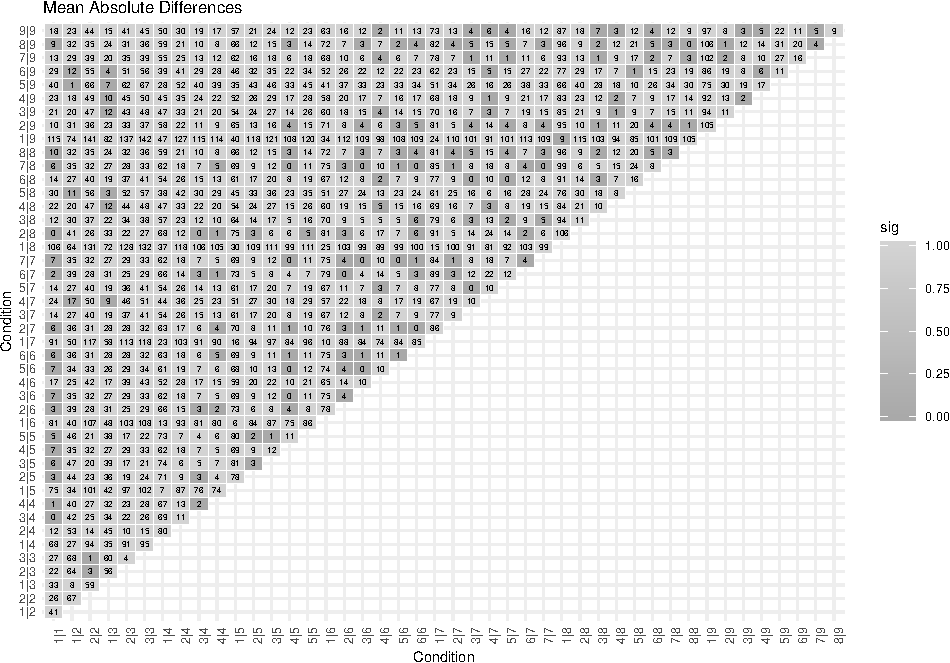
\includegraphics{Entropy_typing_draft_files/figure-latex/typing_mean_iksis_comparisons-1.pdf}
\caption{}
\end{figure}

For each subject, we calculated mean IKSIs as a function of letter
position and word length. The letter position and word length factors
were not factorially crossed. To determine whether there were
differences among the means we submitted the means to a single factor
repeated measures design with 45 levels (e.g., letter
position\textbar{}word length: 1\textbar{}1, 1\textbar{}2, 2\textbar{}2,
\ldots{} 9\textbar{}9). Figure 1 shows mean IKSIs collapsed over
subjects, as a function of letter position and word length.

The omnibus test indicated differences among the means were not likely
due to chance, F (44,15180) = 276.74, MSE = 1,269.66, p \textless{}
.001. Visual inspection of figure X shows several trends across the
means consistent with first-letter slowing and mid-word slowing reported
by Ostry (1983).

Our more important aim was to determine whether variation among these
means can be explained by variation in letter uncertainty. For this
reason we do not exhaustively discuss all of the possible 990
differences among these 45 conditions. Nevertheless, we conducted all
990 comparisons using bonferroni corrected paired samples t-tests. The
results are displayed in Figure 1B graphs the absolute mean differences
between conditions using light gray to indicate comparisons where, p
\textless{} .05/990 = .0000505. The overwhelming majority of comparisons
showed differences unlikely to be produced by chance. This demonstrates
systematic effects of letter position and word length on mean
interkeystroke interval.

\subsection{Letter Uncertainty by position and word
length}\label{letter-uncertainty-by-position-and-word-length}

The primary question of interest was whether natural variation in letter
uncertainty explains variance in mean IKSI by position and word length.
We estimated letter uncertainty by position and word length from
Google's Ngram database \url{https://books.google.com/ngrams}, which
provides frequency counts of letters and words occuring in Google's
massive corpus of millions of digitized books. Letter frequency counts
for letters a to z, for each position in words from length one to nine,
were obtained from Peter Norvig's website
\url{http://norvig.com/mayzner.html}.

For each letter frequency distribution, we computed Shannon's H
(entropy) to quantify letter uncertainty. We converted each letter
frequency distribution to a probability distribution then calculated H
for each distribution. Figure 3 displays estimates of letter uncertainty
(H) as a function of letter position and word length. Visual inspection
of the graph shows that variation in letter uncertainty maps closely
onto variation in mean IKSI (Figure 1) as a function of position and
word length. In particular, letter uncertainty and mean IKSI for
position one as a function of word length appear highly similar. And for
the remaining positions, letter uncertainty shows an inverted U- shape
with greater letter uncertainty in the middle rather than the beginning
and endings of words. This suggests that natural variation of letter
uncertainty across position and word in English may account for aspects
of the first-letter and mid-word slowing phenomena in typing.

\subsection{Letter Uncertainty and Mean
IKSI}\label{letter-uncertainty-and-mean-iksi}

If the Hick-Hyman law applied to continuous typing we would expect a
neat linear relationship between mean IKSIs and letter uncertainty.
Figure 4 shows a plot of mean IKSIs taken from all positions and word
lengths against letter uncertainty. The scatterplot shows a general
trend for mean IKSI to increase as a function of letter uncertainty.

\begin{figure}[htbp]
\centering
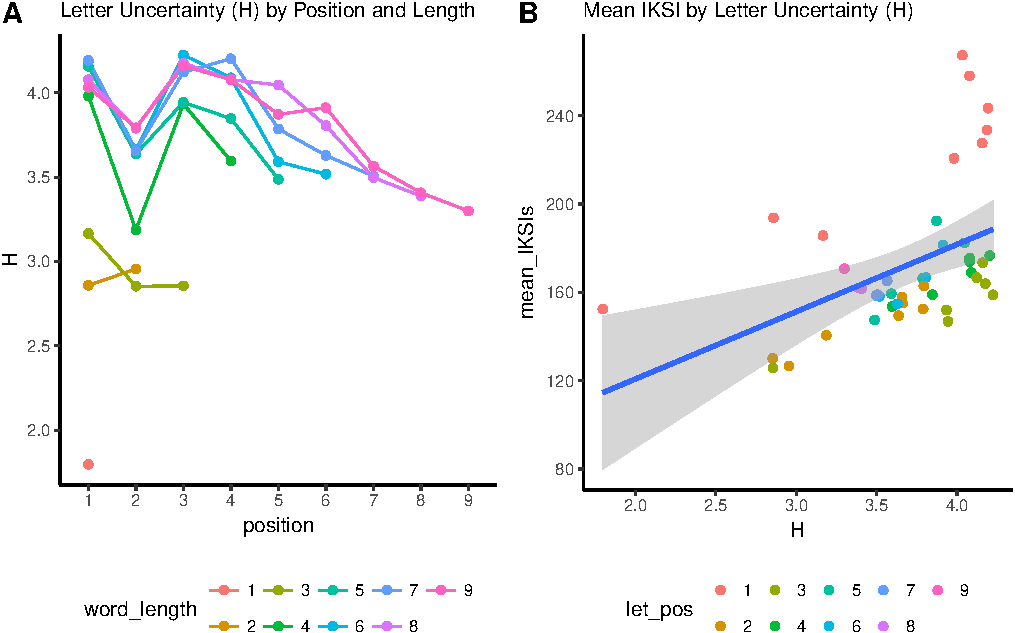
\includegraphics{Entropy_typing_draft_files/figure-latex/letter_uncertainty_by_IKSI-1.pdf}
\caption{}
\end{figure}

A linear regression with group mean IKSIs (collapsed over subjects) as
the dependent variable, and letter uncertainty as the independent
variable showed a significant positive trend, F(1, 43) = 11.82, p =
0.0013, \(R^2 =\) 0.22 ( meanIKSI = 59.75 \(+\) 30.49 \(* H\) ). We also
conducted separate linear regressions for each subject and found similar
results. For example, the mean correlation was r = 0.44 (SE = 0.0085);
mean \(R^2\) = 0.22 (SE = 0.0072); and mean p = 0.047 (SE = 0.0072).

\subsection{Interim Discussion}\label{interim-discussion}

We can conclude that letter uncertainty as a function of position and
length explains a small amount variation in mean IKSIs during continuous
typing. The present analysis does not provide strong evidence that a
process sensitive to letter uncertainty causes both first-letter and
mid-word slowing. For example, all of the first position mean IKSIs are
longer than mean IKSIs for other positions at comparables levels of
letter uncertainty. And, a linear regression on the group mean IKSIs
including letter uncertainty and position (first letter vs.~other
letter) as independent variables explains much more variance, \(R^2\) =
0.86, p \textless{} .001, than the regression only including letter
uncertainty.

This pattern invites a dual-process interpretation. For example,
first-letter slowing could be explained by a planning process that
increases first position IKSIs as a function of word length. Longer
words have more letters, thus plan construction and buffering is assumed
to take more time before sequence production begins. At the same time,
the finding that letter uncertainty does explain some variance in mean
IKSI across position suggests that sequence production is also
influenced by a process sensitive to letter uncertainty.

\subsection{Letter Uncertainty by position, word length, and n-1 letter
identity}\label{letter-uncertainty-by-position-word-length-and-n-1-letter-identity}

Determining whether first-letter and mid-word slowing could emerge from
a process sensitive to letter uncertainty depends on how letter
uncertainty is calculated. Letter uncertainty can be calculated from any
discrete probability distribution of letters. In the previous section we
somewhat arbitrarily calculated letter uncertainty separately for each
letter position in words of length one to nine. However, the number of
alternative schemes is vast. For example, we could further
conditionalize our postion by word length probability distributions by
the letter identities of letters occuring in any position n-1 to n-x, or
n+1 to n+y of a specific position. Furthermore, we could conditionalize
letter distributions upon any permissible number of preceding or
succeeding n-grams (groups of letters).

Although an exhaustive calculation of letter uncertainty is beyond the
scope of this paper, we nevertheless took one further step and
calculated letter uncertainty by position and word length,
conditionalizing upon n-1 letter identity. Fortunately, Norvig
(\url{http://norvig.com/mayzner.html}) also provided bigram frequency
counts from the Google Ngram corpus as a function of position and word
length. We calculated letter uncertainty in the following manner. First
position letters have no preceding letter, so H as a function of word
length was identical to our prior calculation. For letters in positions
two to nine, for all word lengths, we calculated H for every n-1 letter
identity, and then took the mean H for each position and length. For
example, the second position of a two-letter word has a maximum of 26
letter probability distributions, one for each possible n-1 letter (a to
z). We calculated H for all n-1 distributions, then took the mean H as
our measure of letter uncertainty for each position and word length.
Figure X shows mean H conditionalized by n-1 letter identity, as a
function of letter position and word length.

\begin{figure}[htbp]
\centering
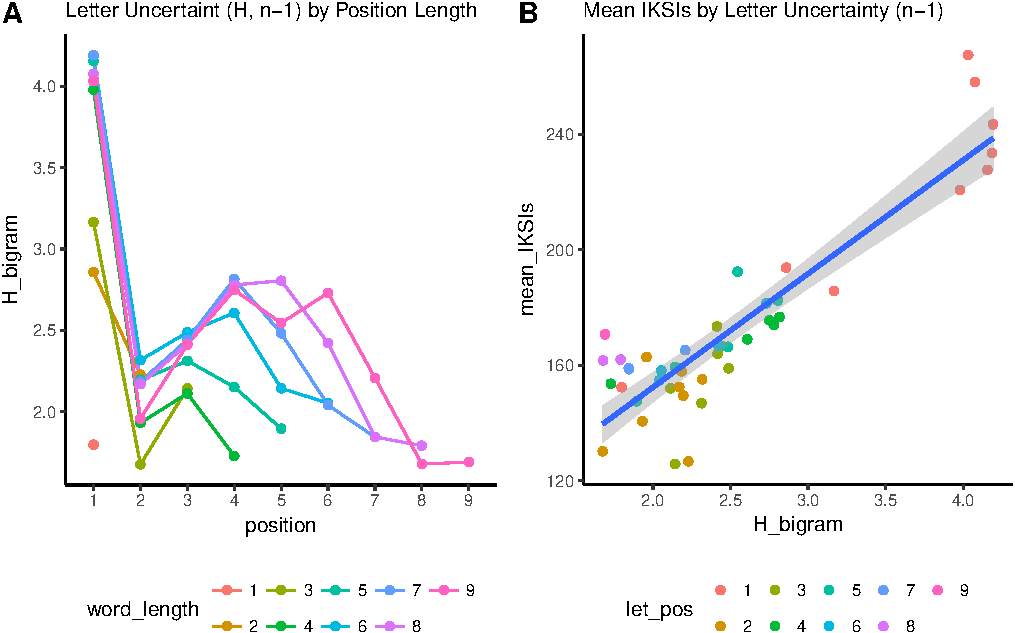
\includegraphics{Entropy_typing_draft_files/figure-latex/letter_uncertainty_bigram-1.pdf}
\caption{}
\end{figure}

Unsurprisingly, letter identity becomes more predictable when n-1 letter
identity is known. Compared to the letter uncertainty measures in Figure
X, we see that H for letters in positions two to nine is much lower when
n-1 letter identity is taken into account. More important, the pattern
of H in Figure X much more closely resembles the pattern of mean IKSIs
in Figure X.

Figure X displays a scatterplot of mean IKSIs as a function of letter
uncertainty conditionalized by letter n-1 identity across positions and
word length. A linear regression on mean IKSIs using our new measure of
letter uncertainty as the independent variable showed a strong positive
relationship, F(1, 43) = 182.44, p = 4.5e-17, \(R^2 =\) 0.81 ( meanIKSI
= 73.72 \(+\) 39.31 \(* H\) ).

\section{An instance-based model}\label{an-instance-based-model}

We have shown that variation in mean IKSIs as a function of letter
position and word length can be well explained by natural variation in
letter uncertainty conditionalized by letter n-1 identity by letter
position and word length. This finding licenses consideration of the
claim that first-letter and mid-word slowing are caused by a single
process sensitive to letter uncertainty. However, the plausibility of
this causal claim is empty in the absence of a working process model.
Next, we establish theoretical plausibility by showing that letter
uncertainty influences on performance can be explained in terms of
Logan's (1988) instance-based memory model of automatization.

Instance theory provides an account of how performance becomes
automatized with practice. We will show instance theory's memory process
also develops sensitivity to uncertainty in the stimuli it encounters
over practice. More specifically, instance theory's predictions for
performance are nearly identical to the hick-hyman law which posits that
reaction times are a linear function of the uncertainty in a choice set.

Instance theory models learning as a function of practice in terms of
cue-driven retrieval of stored memory traces (like other global memory
models, Eich, 1982; Hintzman, 1988; Humphreys, Pike, Bain, \& Tehan,
1989). A new unique trace is preserved in memory every time a response
is given to a stimulus. When a familiar stimulus is encountered again,
it automatically triggers the retrieval of all stored instances of the
stimulus. The timing of the memory-based response to a current stimulus
is treated as a race. Whichever memory trace is retrieved first wins the
race. As a result, the memory-based reaction time to respond to a
stimulus is determined by the retrieval time associated with the fastest
memory trace for that stimulus. The retrieval times for every memory
trace are assumed to vary, and can be sampled from any desired
distribution.

Instance theory models practice based performance speed-ups in terms of
sampling extreme values from a growing retrieval time distribution. As
the number of memory traces grows the range of the retrieval time
distribution also grows, such that he minimum value of the distribution
(fastest retrieval time) is more likely to be smaller for distributions
with more than fewer memory traces. As a result, reaction times will
tend to be faster for more practiced than less practiced stimuli,
because more practiced stimuli have a better chance of retrieving a fast
memory response than less practiced stimuli.

We can now draw a more transparent connection between instance theory
and information theory: they both summarize the same frequency
distributions. Information theory provides H as a summary statistic of
any discrete probability distributions. Empirical probability
distributions for natural occuring stimuli, such as letters, are found
by counting stimulus frequencies, and then dividing a stimulus frequency
distribution by it's sum. Instance theory encodes the frequency
distributions, and summarizes them at retrieval. It predicts
monotonically decreasing RTs as a function of stimulus frequency.
Instance theory predictions for a set of stimuli should concord with H
by taking the grand mean of the predicted RTs for all choices in a set.
We demonstrate these relationships by monte-carlo simulation.

We modeled instance theory predictions for keystroke production times as
a function of letter position and word length, for typing natural
english text. We treated all 26 letters that could possibly occur in any
position for any word length as completely unique and independent
stimuli. We modeled the structure of natural english using the 45 letter
probability distributions derived from Norvig's letter frequence counts
by position and word length, from Google's Ngram corpus.

Keystroke times for specific letters were simulated as a function of
trace frequency by monte-carlo simulation. We assumed that the retrieval
time distribution for each stimulus was sampled from a normal
distribution with mean = 500, and standard deviation = 100. Using R, we
sampled retrieval times from the normal distribution n times, where n
was the current number of memory traces for a given letter. Then we took
the minimum value from the sampling distribution as the reaction time.
We repeated this process 1000 times to estimate the expected mean
reaction time (expected minimum retrieval time) for the given frequency
value. In this way, we estimated mean keystroke production times for
every letter position across different word lengths. Last, we evaluated
model predictions across four practice intervals.

Figure X displays the instance model predictions, across increasing
amounts of practice, for mean keystroke production times as a function
of letter position and word length. As expected, simulated keystroke
times shorten with practice. More imporant, at each stage in practice,
simulated keystroke times show the same qualitative pattern of variation
across letter postion and word length. Notably, these appear very
similar to human typing performance, and to letter uncertainty as a
function of position and word length. We conducted linear regressions on
simulated mean typing times using letter uncertainty as the independent
variable. We found that letter uncertainty nearly perfectly explains the
variance in simulated keystroke time, with \(R^2\) tending toward 1 with
practice.

We point out that the pattern of instance theory predictions for mean
reaction time for any set of choice stimuli will be identical to the
uncertainty, measured by H, for those sets of choices. This means that
instnce theory is a process model of the hick-hyman law, and it inherits
both the successess and failures of information theoretic
interpretations of performance.

\section{General Discussion}\label{general-discussion}

Using data from a large N study of continuous typing performance, we
reproduced Ostry's (1983) demonstration that mean interkeystroke
interval systematically varies as a function of letter position and word
length. We proposed that variation in mean IKSI could be caused by
general learning process sensitive to letter uncertainty across position
and word length. We calculated letter uncertainty in natural english
from Google's large corpus of digitized text, and showed that it can
explain a large portion of the variance (\$R\^{}2 = \$ 0.86) in mean
IKSI. Finally, we show that instance theory (Logan, 1988) succesfully
models how a general learning and memory process could produce typing
performance that is constrained by letter uncertainty. The take home
message is that specialized planning processes for motor sequencing in
typing are sufficient, but not necessary to explain variation in mean
IKSI as a function of letter position and word length; and, that a
general learning process provides a more parsimonious account of the
data.

\subsection{Inferential limitations}\label{inferential-limitations}

We have developed a falsifiable causal theory of variation in keystroke
dynamics across position and word length for continuous typing of
natural english text. However, we are presently limited in the strength
of our causal conclusions. Theoretically, we can conclude, by deduction,
that an instance model predicts IKSIs will vary as a function of H.
Empirically, we have shown correlational evidence that H explains a
large portion of the variance in IKSIs across position and word length.
However, in this study we did not directly manipulate letter uncertainty
by position and word length. Instead, we view the present study as a
natural quasi-experimental design, where typists are presumed to be
exposed to natural varying conditions of letter uncertainty across
position and word length over the course of their experience with
typing.

The theory could be tested further in a few ways. For example, if letter
uncertainty as a function of letter position and word length varies in
different ways across languages, then IKSIs by position and length
should also vary across natural languages, following the
language-specific pattern of H. Experiments with non-word strings that
manipulate the pattern of letter uncertainty across position and word
length could also be conducted. Here, IKSIs by position and length
should always correspond to the pattern of H. However, it is unclear
whether expert typists already familiar with typing in one language
would rapidly adapt their performance to the novel letter uncertainty
contraints (but see, Crump and Logan (2010), for a demonstration that
recent episodic experience influences IKSI).

\subsection{Instance theory and skilled sequential
action}\label{instance-theory-and-skilled-sequential-action}

Our findings fit well with prior work showing instance-based influences
over typing performance, and sequencing in general. For example,
borrowing from (Masson, 1986), Crump and Logan (2010) showed that recent
episodic experience with typing subsets of letters shortens IKSIs for
practiced letters, and suggested that letter typing is driven by
instance-based retrieval process. Behmer and Crump (2017) showed that
instance theory uniquely predicts, compared to a serial recurrent
network model (Cleeremans, 1993; Elman, 1990), changes in sensitivity to
letter, bigram, and trigram frequency as a function of typing expertise.
Gordon D. Logan (In Press) has extended instance-based model to account
for context-driven automatization over response scheduling typing.
Finally, outside of the domain of typing, Jamieson and Mewhort (2009)
showed that an instance-based account explains performance in the serial
reaction time task (Nissen \& Bullemer, 1987), a well controlled
laboratory sequencing task.

The limitations of the instance-based approach higlight open questions.
For example, the core assumption that trace-based retrieval times
determine memory-based performance implies that practice, in and of
itself, is not necessary for automatization. Practice is one route to
automatization because it increases the population of traces, thereby
increasing the likelihood the population contains fast retrieval times
for traces that could support automatization. Indeed, instance theory
allows for single-trial automatization, which occurs when the first
trace sampled into memory happens to have a very fast retrieval time
(for a demonstration see, Gordon D. Logan and Klapp (1991)). However,
instance theory does not lay bare the factors determining how trace
encoding processes could reliably record fast traces to optimize the
automatization process.

Nevertheless, instance theory could provide theoretically optimized
practice schedules for learning to type in an optimal manner. For
example, an instance model could be trained to type any set of texts,
and learning curves plotting mean IKSI as a function of text and
practice would show how typing skill depends on letter uncertainty in
the trained text. The applied question for everyday typists is to
determine which training texts (e.g., natural texts, random letter
texts, parametrically scaled approximations to natural text) provide
optimal transfer of automatized typing performance to natural texts.

Although instance theory allows for single-trial automatization, we
suspect a magic encoding wand will not replace extended practice for
automatizing typing performance. Instead, instance theory also higlights
the critical role of context for automatization. As previously,
mentioned typing performance at the keystroke level is highly dependent
on the immediate letter context (Gentner, 1982; Salthouse, 1986;
Shaffer, 1973). Instance theory explains context dependency by assuming
traces are stored in a context-dependent fashion. A limitation of
instance theory is that it is agnostic, and possibly gratuitous, in
specifying which cues in enivronment are used as contexts to
conditionalize trace storage and retrieval. Our findings suggest at a
minimum, that typists are sensitive to letter uncertainty in a deeply
context-specific manner, including context specified by letter position,
word length, and letter n-1 identity. The implication is that experience
with typing letters in all functional contexts is required for
automatizing letter typing, perhaps necessiting extended practice as
means to experience all of the contexts.

An important remaining question is to characterize the functional
envelope of contextual cues mediating retrieval of stored instances in
typing. For example, letter identities or ngram units at positions n-x
to n+y may also be effective contextual cues mediating retrieval
keystroke retrieval times. We suggest that information theory may be
used to characterize the natural horizon of structure surrounding
individual letters. For example, when we took letter n-1 identity into
account, measures of H across letter position and word length were
dramatically reduced from 4.7, because n-1 letter identity is highly
predictive of letter n identity. However, we expect that expanding the
calculation of letter uncertainty to include more preceding and
succeeding letter identities will show the natural envelope of H. In
other words, letter identities at some remote location will eventually
be unpredictive of letter identities at the current position. We think
it would be telling if the natural span of the letter uncertainty
envelope maps onto the known rate limiting eye-hand copying spans in
typing (Gordan D. Logan, 1983). For example, typing speed slows down as
preview of upcoming letters is restricted (Hershman \& Hillix, 1965),
and it remains unknown how the size of the preview window corresponds to
the natural span of letter uncertainty conditionalized on succeeding
letters. Some rate-limiting aspects of limited preview may not reflect
internal processing limitations (McLeod \& Hume, 1994; Pashler, 1994a,
1994b), but external constraints on the value of the information in the
preview window.

\section{Broader implications and
Conlusions}\label{broader-implications-and-conlusions}

We are optimistic that the tools and approach used here could be
succesfully applied to other domains beyond skilled typing. We found
that information theory, despite it's flexibility, was a useful measure
of structure in the typing environment. Generalist models of cognitive
processes assume that cogniton arises through interaction with a
structured environment. In addition to specifying the learning and
memory rules that extract the structure, it is equally valuable to
improve measurement of structure in the environment. Information theory
provides one flexible measurement framework for describing the amount of
correlated or redundant structure within any set of units in the
environment. When applied judiciously, it becomes theoretically possible
to define the limits of what a general learning process could learn from
an environment. These limits could be useful for testing generalist
theories against special process theories, especially when it can be
shown that a cognitive process has more knowledge than the structure in
an environment could provide.

Information theory spurred the cognitive revolution (Hick, 1952; Hyman,
1953; Miller, 1956), and although it was roundly criticized (see
{\textbf{???}}), we think it has descriptive value useful for
characterizing the structure in big data turning the next revolution
(Griffiths, 2015). Our demonstration of correspondence between instance
theory (Gordon D. Logan, 1988) and measures of uncertainty adds to the
process models capable of accounting for uncertainty mediated phenomena
(for a review see, {\textbf{???}}), and offers principled and
falsifiable predictions for future work.

\newpage

\section{References}\label{references}

\begingroup
\setlength{\parindent}{-0.5in} \setlength{\leftskip}{0.5in}

\hypertarget{refs}{}
\hypertarget{ref-R-papaja}{}
Aust, F., \& Barth, M. (2018). \emph{papaja: Create APA manuscripts with
R Markdown}. Retrieved from \url{https://github.com/crsh/papaja}

\hypertarget{ref-R-magrittr}{}
Bache, S. M., \& Wickham, H. (2014). \emph{Magrittr: A forward-pipe
operator for r}. Retrieved from
\url{https://CRAN.R-project.org/package=magrittr}

\hypertarget{ref-behmer_crunching_2017}{}
Behmer, L. P., \& Crump, M. J. C. (2017). Crunching big data with finger
tips: How typists tune their performance towards the statistics of
natural language. In M. N. Jones (Ed.), \emph{Big Data in Cognitive
Science} (pp. 319--341).

\hypertarget{ref-clark_supersizing_2008}{}
Clark, A. (2008). \emph{Supersizing the mind: Embodiment, action, and
cognitive extension}. OUP USA. Retrieved from
\url{https://books.google.com/books?hl=en\&lr=\&id=n5wRDAAAQBAJ\&oi=fnd\&pg=PR9\&dq=andy+clark\&ots=_Cpl448Qox\&sig=SC8xkxJaEf7G8EZaGPS0zSDEQX8}

\hypertarget{ref-cleeremans_mechanisms_1993}{}
Cleeremans, A. (1993). \emph{Mechanisms of implicit learning
connectionist models of sequence processing}. Cambridge, Mass.: MIT
Press.

\hypertarget{ref-R-Crump}{}
Crump, M. (2017). \emph{Crump: Crump lab functions}.

\hypertarget{ref-crump_episodic_2010}{}
Crump, M. J. C., \& Logan, G. D. (2010). Episodic contributions to
sequential control: Learning from a typist's touch. \emph{Journal of
Experimental Psychology: Human Perception and Performance},
\emph{36}(3), 662--672.
doi:\href{https://doi.org/10.1037/a0018390}{10.1037/a0018390}

\hypertarget{ref-R-data.table}{}
Dowle, M., \& Srinivasan, A. (2017). \emph{Data.table: Extension of
`data.frame`}. Retrieved from
\url{https://CRAN.R-project.org/package=data.table}

\hypertarget{ref-R-RcppZiggurat}{}
Eddelbuettel, D. (2017). \emph{RcppZiggurat: 'Rcpp' integration of
different ``ziggurat'' normal rng implementations}. Retrieved from
\url{https://CRAN.R-project.org/package=RcppZiggurat}

\hypertarget{ref-R-Rcpp_b}{}
Eddelbuettel, D., \& Balamuta, J. J. (2017). Extending extitR with
extitC++: A Brief Introduction to extitRcpp. \emph{PeerJ Preprints},
\emph{5}, e3188v1.
doi:\href{https://doi.org/10.7287/peerj.preprints.3188v1}{10.7287/peerj.preprints.3188v1}

\hypertarget{ref-R-Rcpp_a}{}
Eddelbuettel, D., \& François, R. (2011). Rcpp: Seamless R and C++
integration. \emph{Journal of Statistical Software}, \emph{40}(8),
1--18.
doi:\href{https://doi.org/10.18637/jss.v040.i08}{10.18637/jss.v040.i08}

\hypertarget{ref-eich_composite_1982}{}
Eich, J. M. (1982). A composite holographic associative recall model.
\emph{Psychological Review}, \emph{89}(6), 627--661.

\hypertarget{ref-elman_finding_1990}{}
Elman, J. L. (1990). Finding structure in time. \emph{Cognitive
Science}, \emph{14}(2), 179--211.

\hypertarget{ref-fodor_modularity_1983}{}
Fodor, J. A. (1983). \emph{The modularity of mind: An essay on faculty
psychology}. Cambridge, Mass.: MIT Press.

\hypertarget{ref-GentnerEvidencecentralcontrol1982}{}
Gentner, D. R. (1982). Evidence against a central control model of
timing in typing. \emph{Journal of Experimental Psychology: Human
Perception and Performance}, \emph{8}(6), 793--810.
doi:\href{https://doi.org/10.1037/0096-1523.8.6.793}{10.1037/0096-1523.8.6.793}

\hypertarget{ref-griffiths_manifesto_2015}{}
Griffiths, T. L. (2015). Manifesto for a new (computational) cognitive
revolution. \emph{Cognition}, \emph{135}, 21--23.

\hypertarget{ref-grudin_digraph_1982}{}
Grudin, J. T., \& Larochelle, S. (1982). \emph{Digraph Frequency Effects
in Skilled Typing.} DTIC Document. Retrieved from
\url{http://oai.dtic.mil/oai/oai?verb=getRecord\&metadataPrefix=html\&identifier=ADA112926}

\hypertarget{ref-heath_stochastic_1990}{}
Heath, R. A., \& Willcox, C. H. (1990). A stochastic model for
inter-keypress times in a typing task. \emph{Acta Psychologica},
\emph{75}(1), 13--39.

\hypertarget{ref-HershmanDataProcessingTyping1965}{}
Hershman, R. L., \& Hillix, W. A. (1965). Data Processing in Typing:
Typing Rate as a Function of Kind of Material and Amount Exposed1.
\emph{Human Factors: The Journal of the Human Factors and Ergonomics
Society}, \emph{7}(5), 483--492.

\hypertarget{ref-hick_rate_1952}{}
Hick, W. E. (1952). On the rate of gain of information. \emph{Quarterly
Journal of Experimental Psychology}, \emph{4}(1), 11--26. Retrieved from
\url{http://www.tandfonline.com/doi/abs/10.1080/17470215208416600}

\hypertarget{ref-hintzman_judgments_1988}{}
Hintzman, D. L. (1988). Judgments of frequency and recognition memory in
a multiple-trace memory model. \emph{Psychological Review},
\emph{95}(4), 528.

\hypertarget{ref-humphreys_global_1989}{}
Humphreys, M. S., Pike, R., Bain, J. D., \& Tehan, G. (1989). Global
matching: A comparison of the SAM, Minerva II, Matrix, and TODAM models.
\emph{Journal of Mathematical Psychology}, \emph{33}(1), 36--67.

\hypertarget{ref-hyman_stimulus_1953}{}
Hyman, R. (1953). Stimulus information as a determinant of reaction
time. \emph{Journal of Experimental Psychology}, \emph{45}(3), 188.
Retrieved from \url{http://psycnet.apa.org/journals/xge/45/3/188/}

\hypertarget{ref-JacobyNonanalyticcognitionMemory1984}{}
Jacoby, L. L., \& Brooks, L. R. (1984). Nonanalytic cognition: Memory,
perception, and concept learning. \emph{The Psychology of Learning and
Motivation}, \emph{18}, 1--47.

\hypertarget{ref-jamieson_applying_2009}{}
Jamieson, R. K., \& Mewhort, D. J. K. (2009). Applying an exemplar model
to the serial reaction-time task: Anticipating from experience.
\emph{The Quarterly Journal of Experimental Psychology}, \emph{62}(9),
1757--1783. Retrieved from
\url{http://www.tandfonline.com/doi/abs/10.1080/17470210802557637}

\hypertarget{ref-john_typist:_1996}{}
John, B. E. (1996). TYPIST: A theory of performance in skilled typing.
\emph{Human-Computer Interaction}, \emph{11}(4), 321--355.

\hypertarget{ref-R-ggpubr}{}
Kassambara, A. (2017). \emph{Ggpubr: 'Ggplot2' based publication ready
plots}. Retrieved from \url{https://CRAN.R-project.org/package=ggpubr}

\hypertarget{ref-KolersProceduresmind1984}{}
Kolers, P. A., \& Roediger, H. L. (1984). Procedures of mind.
\emph{Journal of Verbal Learning and Verbal Behavior}, \emph{23}(4),
425--449.

\hypertarget{ref-logan_span_1983}{}
Logan, G. D. (1983). Time, information, and the various spans in
typewriting. In W. E. Cooper (Ed.), \emph{Cognitive aspects of skilled
typewriting} (pp. 197--224).

\hypertarget{ref-logan_toward_1988}{}
Logan, G. D. (1988). Toward an instance theory of automatization.
\emph{Psychological Review}, \emph{95}(4), 492--527. Retrieved from
\url{http://psycnet.apa.org/journals/rev/95/4/492/}

\hypertarget{ref-logan_inpress}{}
Logan, G. D. (In Press). Automatic control: How experts act without
thinking. \emph{Psychological Review}, \emph{TBD}(TBD), TBD.

\hypertarget{ref-logan_hierarchical_2011}{}
Logan, G. D., \& Crump, M. J. C. (2011). Hierarchical control of
cognitive processes: The case for skilled typewriting. In B. H. Ross
(Ed.), \emph{Psychology of Learning and Motivation} (Vol. 54, pp.
1--27). Elsevier. Retrieved from
\href{https://CrumpLab.github.io/CognitionPerformanceLab/CrumpPubs/Logan\%20and\%20Crump\%20-\%202011.pdf}{https://CrumpLab.github.io/CognitionPerformanceLab/CrumpPubs/Logan and Crump - 2011.pdf}

\hypertarget{ref-logan_automatizing_1991}{}
Logan, G. D., \& Klapp, S. T. (1991). Automatizing alphabet arithmetic:
I. Is extended practice necessary to produce automaticity? \emph{Journal
of Experimental Psychology: Learning, Memory, and Cognition},
\emph{17}(2), 179--195.

\hypertarget{ref-massaro_typing_1984}{}
Massaro, D. W., \& Lucas, P. A. (1984). Typing letter strings varying in
orthographic structure. \emph{Acta Psychologica}, \emph{57}(2),
109--131.

\hypertarget{ref-MassonIdentificationtypographicallytransformed1986}{}
Masson, M. E. (1986). Identification of typographically transformed
words: Instance-based skill acquisition. \emph{Journal of Experimental
Psychology: Learning, Memory, and Cognition}, \emph{12}(4), 479.

\hypertarget{ref-mcleod_overlapping_1994}{}
McLeod, P., \& Hume, M. (1994). Overlapping mental operations in serial
performance with preview: Typing. A reply to Pashler. \emph{The
Quarterly Journal of Experimental Psychology}, \emph{47}(1), 193--199.

\hypertarget{ref-R-skimr}{}
McNamara, A., Arino de la Rubia, E., Zhu, H., Ellis, S., \& Quinn, M.
(2018). \emph{Skimr: Compact and flexible summaries of data}. Retrieved
from \url{https://CRAN.R-project.org/package=skimr}

\hypertarget{ref-miller_magical_1956}{}
Miller, G. A. (1956). The magical number seven, plus or minus two: Some
limits on our capacity for processing information. \emph{Psychological
Review}, \emph{63}(2), 81--97. Retrieved from
\url{http://psycnet.apa.org/journals/rev/63/2/81/}

\hypertarget{ref-R-bindrcpp}{}
Müller, K. (2018). \emph{Bindrcpp: An 'rcpp' interface to active
bindings}. Retrieved from
\url{https://CRAN.R-project.org/package=bindrcpp}

\hypertarget{ref-NissenAttentionalrequirementslearning1987}{}
Nissen, M. J., \& Bullemer, P. (1987). Attentional requirements of
learning: Evidence from performance measures. \emph{Cognitive
Psychology}, \emph{19}(1), 1--32.

\hypertarget{ref-R-bit64}{}
Oehlschlägel, J. (2017). \emph{Bit64: A s3 class for vectors of 64bit
integers}. Retrieved from \url{https://CRAN.R-project.org/package=bit64}

\hypertarget{ref-R-bit}{}
Oehlschlägel, J. (2018). \emph{Bit: A class for vectors of 1-bit
booleans}. Retrieved from \url{https://CRAN.R-project.org/package=bit}

\hypertarget{ref-OstryDeterminantsinterkeytimes1983}{}
Ostry, D. J. (1983). Determinants of interkey times in typing.
\emph{Cognitive Aspects of Skilled Typewriting}, 225--246.

\hypertarget{ref-R-Rfast}{}
Papadakis, M., Tsagris, M., Dimitriadis, M., Fafalios, S., Tsamardinos,
I., Fasiolo, M., \ldots{} Lakiotaki, K. (2018). \emph{Rfast: A
collection of efficient and extremely fast r functions}. Retrieved from
\url{https://CRAN.R-project.org/package=Rfast}

\hypertarget{ref-pashler_comment_1994}{}
Pashler, H. (1994a). Comment on McLeod and Hume, overlapping mental
operations in serial performance with preview: Typing. \emph{The
Quarterly Journal of Experimental Psychology}, \emph{47}(1), 201--205.

\hypertarget{ref-pashler_overlapping_1994}{}
Pashler, H. (1994b). Overlapping mental operations in serial performance
with preview. \emph{The Quarterly Journal of Experimental Psychology},
\emph{47}(1), 161--191.

\hypertarget{ref-PinetTypingwritingLinguistic2016}{}
Pinet, S., Ziegler, J. C., \& Alario, F.-X. (2016). Typing is writing:
Linguistic properties modulate typing execution. \emph{Psychonomic
Bulletin \& Review}, \emph{23}(6), 1898--1906.

\hypertarget{ref-proctor_hicks_2018}{}
Proctor, R. W., \& Schneider, D. W. (2018). Hick's law for choice
reaction time: A review. \emph{Quarterly Journal of Experimental
Psychology}, \emph{71}(6), 1281--1299.
doi:\href{https://doi.org/10.1080/17470218.2017.1322622}{10.1080/17470218.2017.1322622}

\hypertarget{ref-R-base}{}
R Core Team. (2017). \emph{R: A language and environment for statistical
computing}. Vienna, Austria: R Foundation for Statistical Computing.
Retrieved from \url{https://www.R-project.org/}

\hypertarget{ref-R-rlist}{}
Ren, K. (2016). \emph{Rlist: A toolbox for non-tabular data
manipulation}. Retrieved from
\url{https://CRAN.R-project.org/package=rlist}

\hypertarget{ref-rumelhart_parallel_1986}{}
Rumelhart, D. E., \& McClelland, J. L. (1986). \emph{Parallel
distributed processing, Explorations in the microstructure of cognition,
Volume 1: Foundations}. Cambridge, Mass. {[}u.a.{]}: MIT Press.

\hypertarget{ref-RumelhartSimulatingskilledtypist1982}{}
Rumelhart, D. E., \& Norman, D. A. (1982). Simulating a skilled typist:
A study of skilled cognitive-motor performance. \emph{Cognitive
Science}, \emph{6}(1), 1--36.

\hypertarget{ref-salthouse_effects_1984}{}
Salthouse, T. A. (1984). Effects of age and skill in typing.
\emph{Journal of Experimental Psychology: General}, \emph{113}(3), 345.

\hypertarget{ref-salthouse_perceptual_1986}{}
Salthouse, T. A. (1986). Perceptual, cognitive, and motoric aspects of
transcription typing. \emph{Psychological Bulletin}, \emph{99}(3),
303--319.

\hypertarget{ref-shaffer_latency_1973}{}
Shaffer, L. H. (1973). Latency mechanisms in transcription.
\emph{Attention and Performance IV}, 435--446.

\hypertarget{ref-shaffer_typing_1968}{}
Shaffer, L. H., \& Hardwick, J. (1968). Typing performance as a function
of text. \emph{The Quarterly Journal of Experimental Psychology},
\emph{20}(4), 360--369.

\hypertarget{ref-Shannonmathematicaltheorycommunication1998}{}
Shannon, C. E., \& Weaver, W. (1998). \emph{The mathematical theory of
communication}. University of Illinois press.

\hypertarget{ref-terzuolo_determinants_1980}{}
Terzuolo, C. A., \& Viviani, P. (1980). Determinants and characteristics
of motor patterns used for typing. \emph{Neuroscience}, \emph{5}(6),
1085--1103.

\hypertarget{ref-van_selst_solution_1994}{}
Van Selst, M., \& Jolicoeur, P. (1994). A solution to the effect of
sample size on outlier elimination. \emph{The Quarterly Journal of
Experimental Psychology}, \emph{47A}, 631--650.

\hypertarget{ref-vinson_quantifying_2017}{}
Vinson, D. W. (2017). \emph{Quantifying Context and its Effects in Large
Natural Datasets} (PhD Thesis). University of California, Merced.

\hypertarget{ref-R-ggplot2}{}
Wickham, H. (2009). \emph{Ggplot2: Elegant graphics for data analysis}.
Springer-Verlag New York. Retrieved from \url{http://ggplot2.org}

\hypertarget{ref-R-dplyr}{}
Wickham, H., Francois, R., Henry, L., \& Müller, K. (2017). \emph{Dplyr:
A grammar of data manipulation}. Retrieved from
\url{https://CRAN.R-project.org/package=dplyr}

\hypertarget{ref-will_linguistic_2006}{}
Will, U., Nottbusch, G., \& Weingarten, R. (2006). Linguistic units in
word typing: Effects of word presentation modes and typing delay.
\emph{Written Language \& Literacy}, \emph{9}(1), 153--176.

\hypertarget{ref-wu_queuing_2008}{}
Wu, C., \& Liu, Y. (2008). Queuing Network Modeling of Transcription
Typing. \emph{ACM Transactions on Computer-Human Interaction},
\emph{15}(1), 1--45.
doi:\href{https://doi.org/10.1145/1352782.1352788}{10.1145/1352782.1352788}

\hypertarget{ref-R-knitr}{}
Xie, Y. (2015). \emph{Dynamic documents with R and knitr} (2nd ed.).
Boca Raton, Florida: Chapman; Hall/CRC. Retrieved from
\url{https://yihui.name/knitr/}

\endgroup






\end{document}
